\section{Data Model and ETL}
\label{sec:data}

\begin{figure}[!h]
\begin{center}
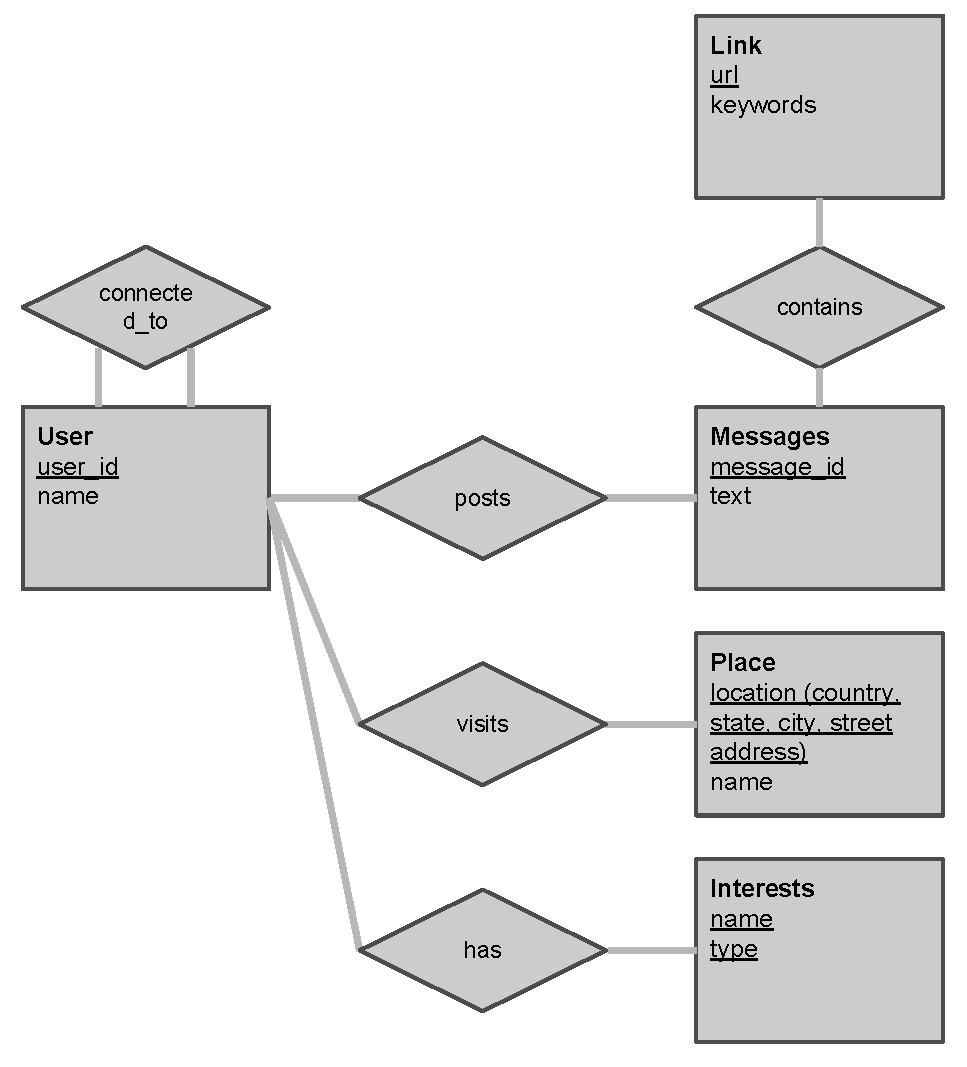
\includegraphics[width=0.5\linewidth]{figs/er-datasource.pdf}
\caption{Entity-Relationship Diagram for Data Sources}
\label{fig:er-datasource}
\end{center}
\end{figure}

In order to efficiently perform computations over data...we define the following
format...
We represent social networking data using the Entity Relationship (ER) diagram
shown in Figure~\ref{fig:er-datasource}.
Conceptually, we see three types of site interactions -- post, profile (has),
and visit

\begin{figure}[!h]
\begin{center}
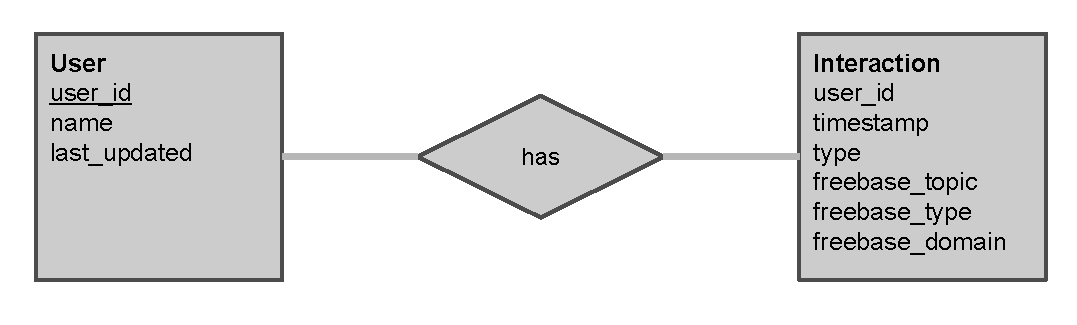
\includegraphics[width=0.5\linewidth]{figs/er-agent.pdf}
\caption{Simplified Entity-Relationship Diagram for Agent Backend}
\label{fig:er-agent}
\end{center}
\end{figure}

Our target data model is shown in Figure~\ref{fig:er-agent}.
We have simplified it for the sake of discussion, 
e.g.\ We end up splitting into three tables for ease of adapting the algorithms to be
specific to data source type and
storing more information, but conceptually it's the same.
